\subsubsection{Context}

Conventional systems neuroscience experiments are typically short in duration
and often place significant constraints on subject behavior to simplify data
analysis.
%
However, these restrictions may limit our ability to observe critical
aspects of brain function and behavior that only manifest in more naturalistic
and extended conditions.

At the Sainsbury Wellcome Centre (SWC) for Neural Circuits and Behaviour, we
are pioneering Naturalistic, Long-Duration, and Continual (NaLoDuCo) foraging
experiments in mice that span weeks to months. During these extended
experiments, we collect high-resolution recordings of both behavioral and
neural activity in naturalistic settings.
%
In collaboration with the Gatsby Computational Neuroscience Unit (GCNU), we are
developing novel analytical methods to interpret this new class of data.

This novel experimental approach will enable researchers to explore neural
mechanisms underlying behavior over extended periods for the first time,
offering the possibility of uncovering insights across a wide range of
phenomena, including long-term behavioral adaptation, neural plasticity, and
learning.
%
The data generated from NaLoDuCo experiments represent an entirely
new resource in neuroscience, with the potential to drive breakthroughs and
discoveries that are beyond the reach of traditional experiments.

Our vision is to empower research centers worldwide to adopt this
groundbreaking approach.
%
However, the scale and complexity of the data generated pose significant
challenges in data acquisition, visualisation, and analysis.
%
In this proposal, we will address these challenges, developing and sharing
openly the necessary expertise, hardware, and software to enable this
transformative type of experimentation on a global scale.

\subsubsection{Focus areas}

Below, we outline the key focus areas we aim to address
(Figure~\ref{fig:focusAreas}), along with their associated challenges.
%
These challenges primarily revolve around the collection and analysis of
continuously recorded, extremely large datasets--on the order of hundreds of
terabytes--gathered from experiments spanning weeks to months.

While experiments in neuroscience that are naturalistic, long-duration, or
continuous have been conducted in the past
\citep[e.g.,][]{jhuangEtAl10,maoEtAl21,volohEtAl23}, to the best of our
knowledge, we are the first to integrate all three of these features in a
single experimental paradigm.
%
This combination introduces unprecedented complexities in data processing, as
we aim to capture behavior and brain activity in their most ecologically valid,
extended, and uninterrupted forms.

The focus areas of the proposed project are (Figure~\ref{fig:focusAreas}):

\begin{description}

    \item[Data Collection \& Management] Efficiently gathering and organizing
        massive datasets over extended periods.

    \item[Data Sharing] Providing easy access to large-scale datasets
        to researchers around the globe using cloud-based technologies.

    \item[Data Visualization] Developing efficient web-based tools to visualize
        very large behavioral and neural datasets.

    \item[Spike Sorting] Assigning spikes to neurons reliably, and tracking
        individual neurons across long-periods of time in real time.

    \item[Data Analysis] Evaluating existing methods, and developing new ones,
        when necessary, to address key problems in behavioral and neural data
        analysis (Figure~\ref{fig:dataAnalysis}).

    \item[Inference-Driven Experimentation] Creating a new type of
        experimentation driven by real-time behavioral and neural inferences.

\end{description}

These focus areas represent key technical and analytical challenges that, once
addressed, will faciliate a transformative shift in neuroscience research.

\begin{figure}
    \begin{center}
        \resizebox{4.0in}{!}{%
            \resizebox{5in}{!}{%
    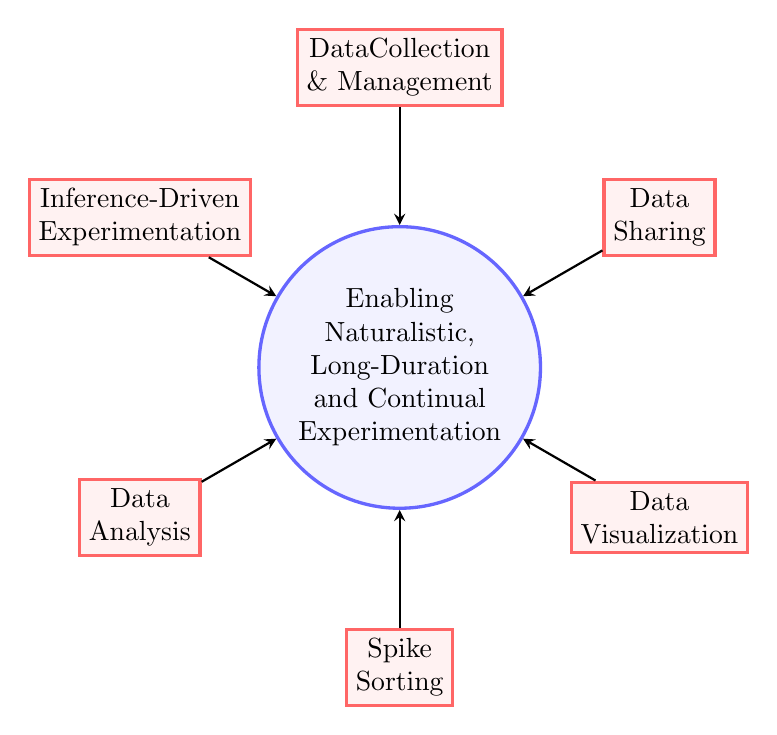
\begin{tikzpicture}[
            node distance=4cm and 1cm,
            centralNode/.style={circle, draw=blue!60, fill=blue!5, very thick,
            minimum size=7mm, align=center},
            itemNode/.style={rectangle, draw=red!60, fill=red!5, very thick,
            minimum size=5mm, align=center},
            arrow/.style={thick, <-, >=stealth},
        ]
        \node[centralNode] (naloducoExp)    {Enabling\\Naturalistic,\\Long-Duration\\and Continual\\Experimentation};
        % \node[itemNode]    (dataCol)        at (naloducoExp) ++(40:2cm) {DataCollection\\\& Management};
            \path (naloducoExp) ++(90:1.5in) node[itemNode] (dataCol) {DataCollection\\\& Management};
            \path (naloducoExp) ++(30:1.5in) node[itemNode] (dataSharing) {Data\\Sharing};
            \path (naloducoExp) ++(330:1.5in) node[itemNode] (dataVis) {Data\\Visualization};
            \path (naloducoExp) ++(270:1.5in) node[itemNode] (spikeSort) {Spike\\Sorting};
            \path (naloducoExp) ++(210:1.5in) node[itemNode] (dataAnalysis) {Data\\Analysis};
            \path (naloducoExp) ++(150:1.5in) node[itemNode] (inferenceDExp) {Inference-Driven\\Experimentation};
        \draw[arrow] (naloducoExp) -- (dataCol);
        \draw[arrow] (naloducoExp) -- (dataSharing);
        \draw[arrow] (naloducoExp) -- (dataVis);
        \draw[arrow] (naloducoExp) -- (spikeSort);
        \draw[arrow] (naloducoExp) -- (dataAnalysis);
        \draw[arrow] (naloducoExp) -- (inferenceDExp);
    \end{tikzpicture}
}

        }
    \end{center}
    \caption{Project theme (blue) and focus areas (red).}
    \label{fig:focusAreas}
\end{figure}

\begin{figure}
    \centering
    \subfloat[]{
        \resizebox{3.0in}{!}{%
            \begin{tikzpicture}[
        node distance=4cm and 1cm,
        behaviorNode/.style={ellipse, draw=cyan!60, fill=cyan!5, very thick,
        minimum size=7mm, align=center},
        problemNode/.style={rectangle, draw=gray!60, fill=gray!5, very thick,
        minimum size=5mm, align=center},
        arrow/.style={thick, <-, >=stealth},
    ]
    \node[behaviorNode] (behavior)    {Behavior};
        \path (behavior) ++(190:1.0in) node[problemNode] (mbpTracking) {Multi\\Body Part\\Tracking};
        \path (behavior) ++(230:1.0in) node[problemNode] (kinematicsInference) {Kinematics\\Inference};
        \path (behavior) ++(310:1.0in) node[problemNode] (statesInference) {State\\Inference};
        \path (behavior) ++(350:1.0in) node[problemNode] (policyInference) {Policy\\Inference};
    \draw[arrow] (behavior) -- (mbpTracking);
    \draw[arrow] (behavior) -- (kinematicsInference);
    \draw[arrow] (behavior) -- (statesInference);
    \draw[arrow] (behavior) -- (policyInference);
\end{tikzpicture}

        }
    }
    \hfill
    \subfloat[]{
        \resizebox{3.0in}{!}{%
            \begin{tikzpicture}[
        node distance=4cm and 1cm,
        neuralNode/.style={ellipse, draw=magenta!60, fill=magenta!5, very thick,
        minimum size=5mm, align=center},
        problemNode/.style={rectangle, draw=gray!60, fill=gray!5, very thick,
        minimum size=5mm, align=center},
        arrow/.style={thick, <-, >=stealth},
    ]
    \node[neuralNode] (neural)    {Neural\\Activity};
        \path (neural) ++(190:1.0in) node[problemNode] (spikeSorting) {Spike\\Sorting};
        \path (neural) ++(230:1.0in) node[problemNode] (latentsInference) {Latents\\Inference};
        \path (neural) ++(310:1.0in) node[problemNode] (stateInference) {State\\Inference};
        \path (neural) ++(350:1.0in) node[problemNode] (decoding) {Decoding};
    \draw[arrow] (neural) -- (spikeSorting);
    \draw[arrow] (neural) -- (latentsInference);
    \draw[arrow] (neural) -- (stateInference);
    \draw[arrow] (neural) -- (decoding);
\end{tikzpicture}

        }
    }
    \caption{Behavioral (a) and neural (b) data analysis problems to address.}
    \label{fig:dataAnalysis}
\end{figure}

